\section{Materiais e Métodos}
\subsection{Materiais}
Para captar e realizar a leitura do ruído eletromagnético foram utilizados uma antena para a captação
e um microcontrolador para a aquisição do valor do ruído captado.
\subsubsection{Arduino UNO}
O Arduino Uno (Fig 1) é uma placa de microcontrolador baseado no ATmega328 (datasheet). Possui 14 pinos de entrada/saída digital (dos quais 6 podem ser usados como saídas PWM), 6 entradas analógicas, um cristal oscilador de 16MHz, uma conexão USB e uma entrada de alimentação uma conexão ICSP.

O microcontrolador foi responsável pela leitura do ruído eletromagnético em uma de suas portas analógicas. O ruído foi então convertido para um valor numérico através do conversor analógico-digital (ADC) presente no Arduino.

\begin{figure}[H]
	\label{fig1}
	\begin{centering}
		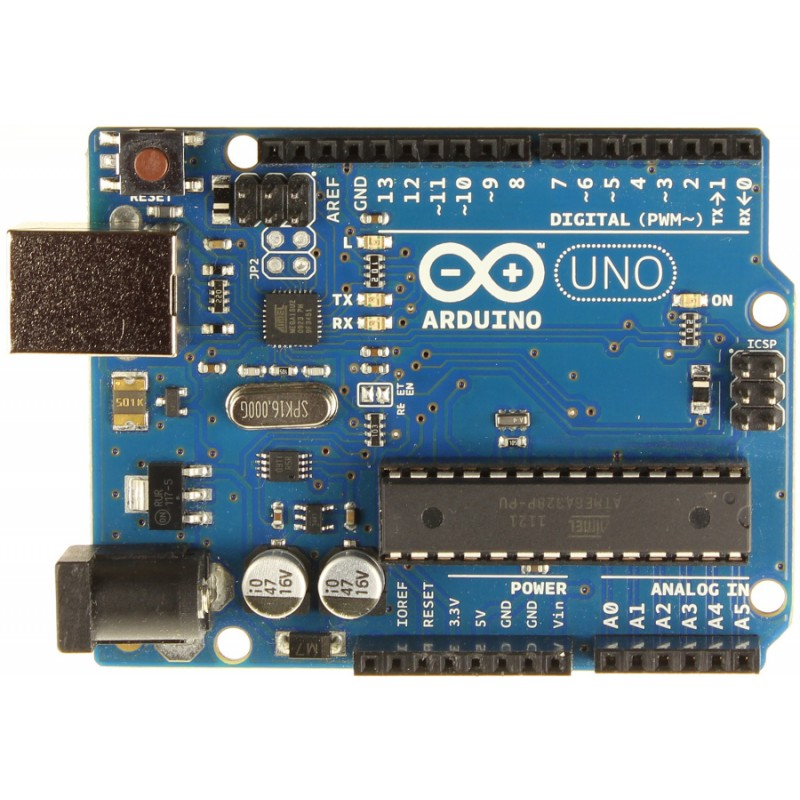
\includegraphics[width = 400pt]{img/arduino.jpg}
		\caption{Arduino UNO}
	\end{centering}	
		
\end{figure}

\subsubsection{Antena}

Foi utilizado um fio de estanho na porta do microcontrolador como aparato para a captação de interferência eletromagnética. A configuração escolhida da antena foi de monopolo de quarto de onda \cite{Balanis2005}.
A frequência captada pela antena é prevista pela equação abaixo:

\begin{equation}
   f = \frac{c}{\frac{L}{4}}
  \end{equation}
sendo $f$ a frequência em Hertz, $c$ a velocidade da luz e $L$ o comprimento da antena. Para uma antena de 8 centímetros, a frequência
captada pela antena é de 15MHz.
 \begin{figure}[H]
 	\label{fig2}
 	\begin{centering}
 		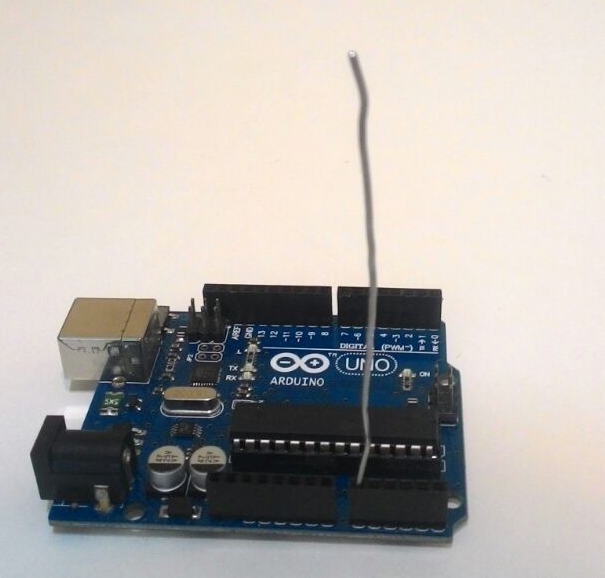
\includegraphics[width = 200pt]{img/arduino2.png}
 		\caption{Arduino UNO com a antena monopolo}
 	\end{centering}	
 		
 \end{figure}

\subsection{Métodos}

Os dados adquiridos pela antena foram tratados no próprio microcontrolador. O ruído ocasionou uma pequena variação de tensão
na porta analógica do Arduino UNO, que foram convertidos para valores na faixa de 0 até 1023. Foram realizadas dez mil leituras, com um
pequeno delay (cerca de 20 milisegundos) entre leituras sucessivas, para evitar ler o mesmo ruído múltiplas vezes. O processamento destas
leituras foi feito de acordo com o algoritmo abaixo.

\begin{algorithm}
\label{alg1}
    \caption{Algoritmo de tratamento de dados}
    \KwIn{Ruído da porta analógica do microcontrolador}
    \KwOut{Sequência de números em base hexadecimal}
    Início\\
    \While(\\
       1.$prev\_value$ $\leftarrow$ valor lido da porta do microcontrolador\\
       2.$value$ $\leftarrow$ próximo valor lido da porta do microcontrolador\\
       3.$d$ $\leftarrow$ $|value - prev\_value|$\\
       4.$d \leftarrow d \mod 16$\\
       5.Imprima $d$ na base hexadecimal){existirem números a serem adquiridos}
       
\end{algorithm}

Este código fornece uma sequência de números na base hexadecimal (0-F). Para as ferramentas de validação do experimento, era necessário
um arquivo binário. Para isso, foi utilizado um código em C para ler os números em hexadecimal e transformá-los em uma sequência binária.

\begin{lstlisting}[caption={Conversão hexa-binário},captionpos=b]
#include <stdio.h>

int main(void) {
	unsigned int a;
	while(scanf("%X", &a) != -1) {
		printf("%c%c", a>>8, a);
	}
	return 0;
}

\end{lstlisting}
